\section{ХОД РАБОТЫ}

\subsection{Текст задания}

Требуется написать программу на языке Prolog, которая будет решать задачу построения расписания.
Условия расписания можно записать следующим образом:
\begin{enumerate}
  \item Первым может быть урок физики или химии.
  \item Вторым может быть урок физики или математики.
  \item Третьим уроком не может быть урок истории.
  \item Четвёртым уроком может быть урок истории или математики.
\end{enumerate}


\subsection{Основные теоретические сведения}

Пролог (англ. Prolog) --- язык и система логического программирования,
основанные на языке предикатов математической логики дизъюнктов Хорна,
представляющей собой подмножество логики предикатов первого порядка.

Основной структурной единицей при программировании на языке Prolog является \textit{клоз}
(от английского clause --- предложение). Клоз имеет общий формат следующего вида:

\texttt{Если (условие) То (результат).}

При написании программ на языке Пролог последнее выражение записывается следующим образом:

\texttt{Результат:-Условие.}

Стоит отметить, что клоз всегда заканчивается точкой.
Условие, как правило, представляет собой несколько
записанных подряд выражений, отделенных друг от друга запятой.
Каждое условие обрабатывается последовательно, в порядке очередности.

Пролог оперирует только логическими отношениями, так что нужно еще придумать,
как систему алгебраических уравнений представить в логической форме.
Запомним терминологию Пролога. Условие (отношение) называется иначе предикатом.

\textit{Предикат} --- это формула с произвольными аргументами, принимающая
только два  значащих значения: \textit{истина} или \textit{ложь}.
Незначащим значением является неопределенность, но в Прологе оно не допустимо.
Аргументы предикатов называются \textit{термами}. Термы могут быть константами,
переменными или функторами (функциями).
Запятая, отделяющая два предиката в клозе, имеет смысл <<\textit{и}>>,
а точка с запятой, отделяющая два предиката в клозе, имеет смысл <<\textit{или}>>.

Стандартными типами аргументов предикатов являются
\texttt{integer, real, string, char, symbol} (\texttt{целый, вещественный,
строковый} --- берется в двойные кавычки,
\texttt{символьный} --- берется в одиночные кавычки;
знаковый записывается без кавычек малыми буквами).

Предикат \texttt{X =:= Y} даёт истину, если записанный слева числовой аргумент равняется
записанному справа числовому аргументу.


\subsection{Особенности разработанной программы}

Составим логические выражения для условия задачи. Введём следующие обозначения:

\begin{itemize}
  \item $\texttt{X}_{i}$ --- $i$-ый по порядку урок химии,
  \item $\texttt{Ф}_{i}$ --- $i$-ый по порядку урок физики,
  \item $\texttt{М}_{i}$ --- $i$-ый по порядку урок математики,
  \item $\texttt{И}_{i}$ --- $i$-ый по порядку урок истории.
\end{itemize}

Из условий задачи можно составить логические выражения:
\begin{equation*}
  \left\{
    \begin{aligned}
      &\texttt{Ф}_1 \lor \texttt{X}_1, \\
      &\texttt{Ф}_2 \lor \texttt{М}_2, \\
      &\texttt{Ф}_3 \lor \texttt{М}_3 \lor \texttt{Х}_3, \\
      &\texttt{М}_4 \lor \texttt{Х}_4. \\
    \end{aligned}
  \right.
\end{equation*}

Запишем дополнительные условия, которые будут гарантировать, что каждый
из предметов встретится в расписании ровно 1 раз:
\begin{minipage}[h!]{0.48\linewidth}
  \begin{equation*}
    \left\{
      \begin{aligned}
        \texttt{Ф}_1 \lor \texttt{Ф}_2 \lor \texttt{Ф}_3 \lor \texttt{Ф}_4, \\
        \texttt{М}_1 \lor \texttt{М}_2 \lor \texttt{М}_3 \lor \texttt{М}_4, \\
        \texttt{Х}_1 \lor \texttt{Х}_2 \lor \texttt{Х}_3 \lor \texttt{Х}_4, \\
        \texttt{И}_1 \lor \texttt{И}_2 \lor \texttt{И}_3 \lor \texttt{И}_4. \\
      \end{aligned}
    \right.
  \end{equation*}
\end{minipage}
\hfill
и
\hfill
\begin{minipage}[h!]{0.48\linewidth}
  \begin{equation*}
    \left\{
      \begin{aligned}
        \texttt{Ф}_1 \lor \texttt{М}_1 \lor \texttt{Х}_1 \lor \texttt{И}_1, \\
        \texttt{Ф}_2 \lor \texttt{М}_2 \lor \texttt{Х}_2 \lor \texttt{И}_2, \\
        \texttt{Ф}_3 \lor \texttt{М}_3 \lor \texttt{Х}_3 \lor \texttt{И}_3, \\
        \texttt{Ф}_4 \lor \texttt{М}_4 \lor \texttt{Х}_4 \lor \texttt{И}_4.
      \end{aligned}
    \right.
  \end{equation*}
\end{minipage}

\vspace{7mm}

% Убираем двойной пробел между equations
\setlength{\belowdisplayskip}{0pt} \setlength{\belowdisplayshortskip}{0pt}

Перейдём от логической формы записи выражений к алгебраической:
\begin{equation*}
  \left\{
    \begin{aligned}
      &\texttt{Ф}_1 + \texttt{X}_1 \ge 1, \\
      &\texttt{Ф}_2 + \texttt{М}_2 \ge 1, \\
      &\texttt{Ф}_3 + \texttt{М}_3 + \texttt{Х}_3 \ge 1, \\
      &\texttt{М}_4 + \texttt{Х}_4 \ge 1, \\
    \end{aligned}
  \right.
\end{equation*}

\begin{minipage}[h!]{0.45\linewidth}
  \begin{equation*}
    \left\{
      \begin{aligned}
        \texttt{Ф}_1 + \texttt{Ф}_2 + \texttt{Ф}_3 + \texttt{Ф}_4 \ge 1, \\
        \texttt{М}_1 + \texttt{М}_2 + \texttt{М}_3 + \texttt{М}_4 \ge 1, \\
        \texttt{Х}_1 + \texttt{Х}_2 + \texttt{Х}_3 + \texttt{Х}_4 \ge 1, \\
        \texttt{И}_1 + \texttt{И}_2 + \texttt{И}_3 + \texttt{И}_4 \ge 1, \\
      \end{aligned}
    \right.
  \end{equation*}
\end{minipage}
\hfill
\begin{minipage}[h!]{0.45\linewidth}
  \begin{equation*}
    \left\{
      \begin{aligned}
        \texttt{Ф}_1 + \texttt{М}_1 + \texttt{Х}_1 + \texttt{И}_1 \ge 1, \\
        \texttt{Ф}_2 + \texttt{М}_2 + \texttt{Х}_2 + \texttt{И}_2 \ge 1, \\
        \texttt{Ф}_3 + \texttt{М}_3 + \texttt{Х}_3 + \texttt{И}_3 \ge 1, \\
        \texttt{Ф}_4 + \texttt{М}_4 + \texttt{Х}_4 + \texttt{И}_4 \ge 1.
      \end{aligned}
    \right.
  \end{equation*}
\end{minipage}

\vspace{7mm}

Для решения задачи на языке Prolog объявим предикаты \texttt{may\_exist(X)}
(передаваемый параметр может принимать значения 0 или 1)
и \texttt{not\_exist(X)} (передаваемый параметр принимает значение~0).

Записанные условия предиката на языке Prolog представлены на рисунке~\ref{lst:predicats}.
\begin{lstlisting}[style=source_code,caption=Условия предиката программы,label=lst:predicats]
 may_exist(P1), may_exist(P2), may_exist(P3), not_exist(P4),
 may_exist(C1), not_exist(C2), not_exist(C3), not_exist(C4),
 not_exist(M1), may_exist(M2), may_exist(M3), may_exist(M4),
 not_exist(H1), not_exist(H2), not_exist(H3), may_exist(H4)
\end{lstlisting}

\newpage

Подробно рассмотрим решение задачи на языке Visual Prolog. Из рисунка~\ref{lst:visual_code} видно,
что исходный код программы можно разделить на несколько секций: \texttt{predicates},
\texttt{clauses} и \texttt{goal}. В секции \texttt{predicates} объявляются предикаты
и аргументы предикатов, если они есть. На рисунке~\ref{lst:} представлена секция \texttt{predicates}
для решаемой задачи.
\begin{lstlisting}[style=source_code,caption=Секция \texttt{predicates} для решаемой задачи,label=lst:predicates]
 nondeterm  equation
 nondeterm  may_exist(integer)
 nondeterm  not_exist(integer)
\end{lstlisting}

Ключевое слово \texttt{nondeterm} означает, что предикат является недетерминированным, то есть
может вырабатывать множество решений посредством бэктрекинга (отката). 

В секции \texttt{goal} обычно объявляют целевой (главный, единственный) предикат, который будет
представлять всю программу как таковую. 

Секция \texttt{clause} содержит клозы, записанные через запятую. Эти клозы выполнются
последовательно, друг за другом. 

Первым выполняется предикат раздела goal --- \texttt{equation}. Система ищет определение
этого предиката в секции \texttt{clauses}. Далее выбирается первое условие из
определения предиката equation --- \texttt{may\_exist(P1)}, и пытается его доказать.  

\textit{Унификацией} называется процесс сопоставления аргументов одноименных предикатов.
В нашем случае это предикаты \texttt{may\_exist(P1)} и \texttt{may\_exist(X):-X=0; X=1}.

При первом обращении к предикату \texttt{may\_exist(X)} переменная \texttt{X} принимает
значение 0. Если это значение не удовлетворяет оставльным предикатам, то
выполняется повторное обращение к предикату \texttt{may\_exist(X)}, и переменная Х
принимает значение 1. Процесс выбора альтернатив на языке Prolog называется
\textit{ветвлением}.

Далее продолжают проверятся все условия по порядку на истинность.
Аргументы всех условий (\texttt{may\_exist(X)} и \texttt{not\_exist(X)})
принимают значение 0. Таким образом программа доходит до доказательства
условия \texttt{P1+P2+P3+P4 >= 1} ($\star$). Попытка доказательства этого условия
заканчивается неудачей, происходит \textit{возврат} в \textit{точку последнего
ветвления}. Точкой последнего ветвления является условие \texttt{may\_exist(H4)}.
Происходит процесс унификации, переменная \texttt{H4} сопоставляется с единицей.
Программа опять пытается доказать истинность условия $\star$. Попытка
заканчивается неудачей, происходит процесс возврата
к условию \texttt{may\_exist(M4)} и так далее.

Для отображения решения задачи в языке GNU Prolog использована функция \texttt{format().}
Результат решения задачи представлен на рисунке~\ref{fig:figure}.

\begin{figure}[h!]
  \centering
  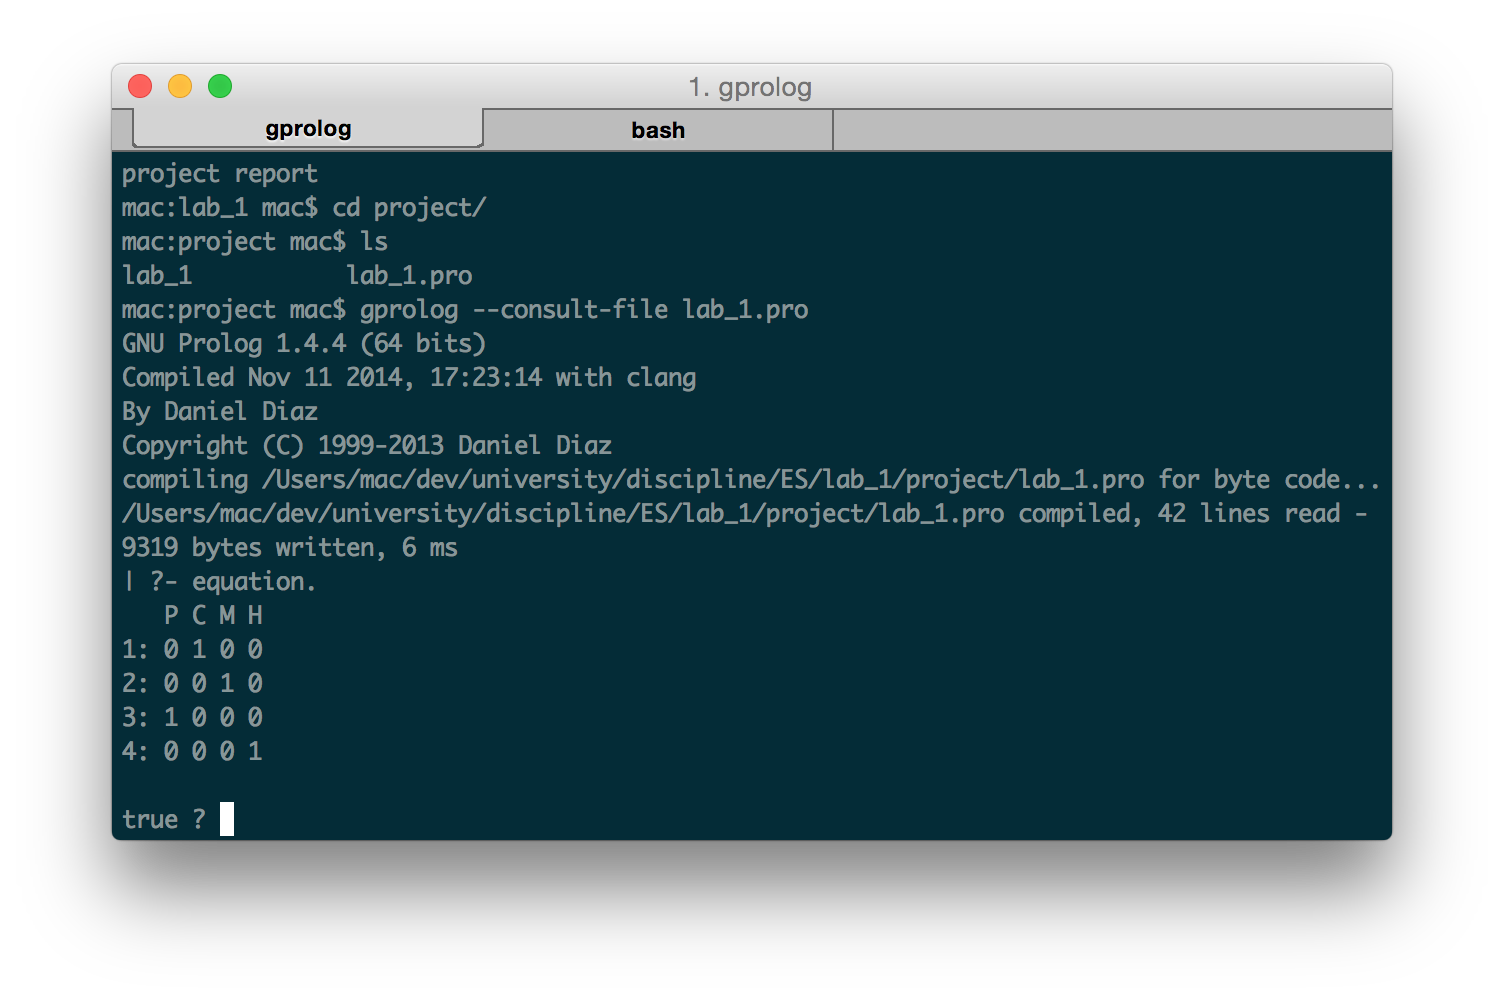
\includegraphics[width=150mm]{img/figure}
  \caption{Результат выполнения программы}
  \label{fig:figure}
\end{figure}

В результате одним из вариантов решения задачи будет следующее расписание:
\begin{enumerate}
  \item Урок химии.
  \item Урок математики.
  \item Урок физики.
  \item Урок истории.
\end{enumerate}

\pagebreak
Исходный код программы на языке GNU Prolog представлен на рисунке~\ref{lst:gnu_code}, а на рисунке~\ref{lst:visual_code} ---
на языке Visual Prolog.

\begin{lstlisting}[style=source_code,caption=Исходный код программы на языке GNU Prolog,label=lst:gnu_code]
 may_exist(X) :-
   X=0; X=1.
 not_exist(X) :-
   X=0.
 equation :-
   may_exist(P1),
   may_exist(P2),
   may_exist(P3),
   not_exist(P4),
   may_exist(C1),
   not_exist(C2),
   not_exist(C3),
   not_exist(C4),
   not_exist(M1),
   may_exist(M2),
   may_exist(M3),
   may_exist(M4),
   not_exist(H1),
   not_exist(H2),
   not_exist(H3),
   may_exist(H4),

   P1 + P2 + P3 + P4 =:= 1,
   C1 + C2 + C3 + C4 =:= 1,
   M1 + M2 + M3 + M4 =:= 1,
   H1 + H2 + H3 + H4 =:= 1,

   P1 + C1 + M1 + H1 =:= 1,
   P2 + C2 + M2 + H2 =:= 1,
   P3 + C3 + M3 + H3 =:= 1,
   P4 + C4 + M4 + H4 =:= 1,
   
   format("   P C M H~N", []),
   format("1: ~w ~w ~w ~w~N", [P1,C1,M1,H1]),
   format("2: ~w ~w ~w ~w~N", [P2,C2,M2,H2]),
   format("3: ~w ~w ~w ~w~N", [P3,C3,M3,H3]),
   format("4: ~w ~w ~w ~w~N", [P4,C4,M4,H4]).
\end{lstlisting}

\newpage

\begin{lstlisting}[style=source_code,caption=Исходный код программы на языке Visual Prolog,label=lst:visual_code]
 predicates
   nondeterm  equation
   nondeterm  may_exist(integer)
   nondeterm  not_exist(integer)         
 goal
   equation.
 clauses equation:-
   may_exist(P1),
   may_exist(P2),
   may_exist(P3),
   not_exist(P4),
   may_exist(C1),
   not_exist(C2),
   not_exist(C3),
   not_exist(C4),
   not_exist(M1),
   may_exist(M2),
   may_exist(M3),
   may_exist(M4),
   not_exist(H1),
   not_exist(H2),
   not_exist(H3),
   may_exist(H4),

   P1 + P2 + P3 + P4 >= 1,
   C1 + C2 + C3 + C4 >= 1,
   M1 + M2 + M3 + M4 >= 1,
   H1 + H2 + H3 + H4 >= 1,
   P1 + C1 + M1 + H1 >= 1,
   P2 + C2 + M2 + H2 >= 1,
   P3 + C3 + M3 + H3 >= 1,
   P4 + C4 + M4 + H4 >= 1,
    
   write("  ","P"," ","C"," ","M"," ","H"), nl,
   write("1:",P1," ",C1," ",M1," ",H1), nl, 
   write("2:",P2," ",C2," ",M2," ",H2), nl, 
   write("3:",P3," ",C3," ",M3," ",H3), nl, 
   write("4:",P4," ",C4," ",M4," ",H4), nl.  

   may_exist(X) :-X=0; X=1.
   not_exist(X) :-X=0.
\end{lstlisting}

\newpage